\chapter{Monadic approach to computational effects}
\label{cpt-monads}

  Monads were initially injected into programming languages context by Moggi as a tool to
  assign a denotational semantics to computational effects~\cite{Moggi:1991:NCM:116981.116984}. Later, Wadler adopted monads as a programming
  paradigm and introduced them into functional programming languages~\cite{Wadler:1992:EFP:143165.143169}. Monads are sometimes referred to as a ``programmable semicolon'' --- a powerful way to construct sequences of computation with possible side effect. Afterwards, even more notions from category theory were given first"/class support in modern programming languages, providing programmers with highly abstract, powerfully expressive and mathematically structured ways to build software.

    \section{Monads in Haskell}

    In Haskell programming language, monads are types that have an instance of \texttt{Monad} type class and satisfy three laws. They are used
    to distinguish pure computations from ones having some kind of side effect:
    mutable state, exceptions, non"/determinism, etc.

    \begin{figure}[h]
    \begin{lstlisting}
class Monad m where
  (>>=)  :: m a -> (a -> m b)   -> m b
  (>>)   :: m a ->  m b         -> m b
  return ::   a                 -> m a
  fail   :: String -> m a
    \end{lstlisting}
    \caption{\texttt{Monad} type class}
    \label{listing:monadClass}
    \end{figure}

    \begin{figure}[h]
    \begin{lstlisting}
return a >>= k                  =  k a
m        >>= return             =  m
m        >>= (\x -> k x >>= h)  =  (m >>= k) >>= h
    \end{lstlisting}
    \caption{Monad laws}
    \label{listing:monadLaws}
    \end{figure}

    The \lstinline{>>=} operation, also known as \emph{monadic bind}, represents
    a mentioned earlier ``programmable semicolon''. It takes a value in a monadic context as it first argument, an action that transforms that value as a second argument and returns a transformed value in the same monadic context.

    Monads have broad usage in functional programming. They are first-class citizens
    in purely-functional languages like Haskell and a wide range of Haskell"/libraries have monadic interface. Mainstream programming languages also
    employ specific monads in a form of build-in language constructions,
    i.e. LINQ in~\cs or optionals in Swift.

    As it was previously said, monads are used to characterise types of computations with a particular side effect. But what if a computation may
    potentially produce two or more effects? Then, means to combine several
    computational effects are needed. Monadic approach provide notion of
    ~\emph{monad transformer}~\cite{Liang:1995:MTM:199448.199528} --- a type that
    may add properties of a given monad to any other. Monad transformers are widely
    used in Haskell to build computations carrying multiple side effects.

    \subsection{Monad transformers}

      Paper~\cite{Liang:1995:MTM:199448.199528} describes a concept of a monad
      transformer --- a building block for types describing computations with
      multiple side effects. Every transformer lets to add a particular
      effect, e.g. mutable state, configuration, exceptions, to a given monad.
      Transformers are put on top of a base monad to form a \emph{monad stack} --- a
      type characterising a computation with multiple side effects. Consider
      an example of a function in a monad combining effects of mutable state and
      configuration (listing~\ref{listing:mtlAdder}).

      \begin{figure}[h]
      \begin{lstlisting}
adder :: StateT String (Reader Int) Int
adder = do
  str <- get
  num <- ask
  return $ num + read str

adder' :: (MonadState String m, MonadReader Int m) => m Int
adder' = ...
      \end{lstlisting}
      \caption{Effectful adder based on monad transformers}
      \label{listing:mtlAdder}
      \end{figure}

      Here \texttt{adder} and \texttt{adder'} describe the same computation, but the first
      function is bounded to specific monad stack, while second just restricts effects
      that the stack ought to provide.

      One characteristic of monad stacks is that ordering of monads is statically encoded
      in the type, so there is no runtime control of effect interaction.
      The Second problem of monad transformers is a need to write a lot of boilerplate
      type class instances, that is, to add a new effect, every possible combination
      of newly added effect with existing ones must be covered with instances to provide
      automatic lifting, thus $\mathcal{O}(n^2)$ instances must be written,
      where $n$ is a number of monad transformers provided by the developing library.

      \begin{figure}[h]
      \begin{lstlisting}
class Monad m => MonadNew a m where
  action1 :: m a
  action2 :: m ()

instance MonadNew m => MonadNew (ExceptT e m) where
  action1 = lift action1
  action2 = lift action2

instance MonadNew m => MonadNew (IdentityT m) where
  action1 = lift action1
  action2 = lift action2

  ...
      \end{lstlisting}
      \caption{Monad classes and instances for lifting}
      \label{listing:mtlLift}
      \end{figure}

      And, finally, monad transformers do not provide a way to express computations that
      produce several homogeneous effects, e.g. two \texttt{State} effects, without
      sacrificing automated lifting.

      Monad transformers are well established abstraction for building modular effectful
      computations. It has been widely accepted by Haskell community and a lot of
      useful libraries have been implemented on top of it. Nevertheless, it has some
      flaws regarding its convenience of use. Lately, algebraic effects and effects
      handlers --- an alternative approach to structuring of effectful computations
      has emerged. It has received wide account in recent
      publications~\cite{DBLP:journals/jlp/BauerP15}~\cite{Kiselyov:2013:EEA:2578854.2503791}
      and has several implementations in programming
      languages~\cite{Kiselyov:2013:EEA:2578854.2503791}~\cite{DBLP:conf/popl/LindleyMM17}.
      The third chapter of this thesis gives a brief overview of two
      implementations: extensible effects library for Haskell and Frank programming language.

  \section{Monadic parsers}
  \label{cpt-parsers:monadic}

    Consider a simple type to represent a parser.

    \begin{figure}[h]
    \begin{lstlisting}
type Parser a = String -> Maybe (a,String)
    \end{lstlisting}
    \caption{Basic parser type}
    \label{listing:maybeParser}
    \end{figure}

    In this representation, parser is a
    function from input stream to possibly non-present accepted result paired
    with the input stream remains.
    Types similar to \texttt{Parser} may be treated as effectful computation.
    One way to represent computations with effects in Haskell
    programming language is to use a concept of \texttt{Monad}. This particular
    type could be made an instance of \texttt{Monad} type class.
    Comprehensive information about properties of parsers like one presented
    above may be found in paper~\cite{monParsing}.

    To make parsers more modular, extend capabilities and improve convenience of
    syntactic analysers, the \texttt{Parser} effect could be factorised into a set of
    primitive effects. Moreover, the set of effect may be extended: it is handy to
    run parsers in a configurable environment or introduce logging.
    This section gives an overview to monadic monad transformers: a monadic framework
    for to build modular effectful computations. As an example, we give a sketch of
    monadic parser combinators library. We do not give the complete implementation
    here, because it's API is fairly similar to one of library implemented in
    Frank programming language and discussed in chapter~\ref{cpt-alg-eff}.

    \subsection{Parser as a monad transformer stack}

      Monad transformer is a concept which lets to enrich a given monad with a
      property of other monad. Multiple monad transformers may be combined
      together to form monad stack, that is, a monad possessing all properties of
      it's components.

      Monadic parser combinators library developed in this work also uses two-layer monad
      stack: state and either,
      where the last one provides effect of possibility of error. Thus, type for parser
      takes a following form.

      \begin{figure}[h]
      \begin{lstlisting}
newtype Parser t a = Parser (
    StateT (ParserState t) (Either (ErrorReport t)) a
  ) deriving ( Functor, Applicative, Monad
             , MonadState (ParserState t)
             , MonadError (ErrorReport t)
             )
      \end{lstlisting}
      \caption{Parser monad stack}
      \label{listing:mtlParser}
      \end{figure}

      This representation of a parsers also is parametrised with type of input stream.
      Types~\texttt{ParserState} and~\texttt{ErrorReport} are algebraic
      data types for representing parser's state and possible analysis errors
      respectively.

      The most low-level primitive which serves as a basis for all parser combinators
      is a parser that consumes a single item from input stream.

      \begin{figure}[h]
      \begin{lstlisting}
item :: TM.TextualMonoid t => Parser t Char
item = do
  state  <- get
  let s = TM.splitCharacterPrefix . remainder $ state
  case s of
    Nothing -> throwError (EmptyRemainder "item",state)
    Just (c,rest) -> do
      let (c,rest) = fromJust s
      put (ParserState {position = updatePos (position state) c
                       , remainder = rest})
      return c
      \end{lstlisting}
      \caption{Unconditional single item consumer}
      \label{listing:mtlParserItem}
      \end{figure}

      More advanced parsers from developed library: conditional consumer and
      given string consumer.

      \begin{figure}[h]
      \begin{lstlisting}
sat :: TM.TextualMonoid t => (Char -> Bool) -> Parser t Char
sat p = do
  state <- get
  x <- item `overrideError` (EmptyRemainder "sat")
  if p x then return x else
    throwError (UnsatisfiedPredicate "general",state)
      \end{lstlisting}
      \caption{Conditional consumer}
      \label{listing:mtlParserSat}
      \end{figure}

      To parse terminals it's convenient to introduce the parser that accepts a
      specific string.

      \begin{figure}[h]
      \begin{lstlisting}
string :: TM.TextualMonoid t => String -> Parser t String
string s = do
  state <- get
  (mapM char s) `overrideError`
    (UnsatisfiedPredicate ("string " ++ s))
      \end{lstlisting}
      \caption{Parser for a static string}
      \label{listing:mtlParserString}
      \end{figure}

      To actually perform parsing, it's necessary to implement a function that
      runs a computation. It's need to be
      pointed out, that order of effect handling is statically encoded in type of
      monad stack.

      \begin{figure}[h]
      \begin{lstlisting}
parse :: TM.TextualMonoid t =>
  Parser t a -> t -> Either (ErrorReport t) (a,ParserState t)
parse (Parser p) s =
  runStateT p (ParserState {remainder = s, position = initPos})
    where initPos = (1,1)
      \end{lstlisting}
      \caption{Running the parser}
      \label{listing:mtlParserParse}
      \end{figure}

      \subsection{Performance benchmark}
      \label{cpt-monads:parsers-bench}

      Here are the result of performance benchmarks of the developed parser
      combinators library. Benchmarks were done using the Haskell Criterion
      library~\cite{criterion}.

      \begin{tabular}{|| c c c||}
        \hline
                      & Estimate & Confidence interval\\
        \hline\hline
        Mean time     & 121 $\mu$s   & [119 $\mu$s, 126 $\mu$s] \\
        $\sigma$      & 10.0 $\mu$s  & [20.2 $\mu$s, 3.84 $\mu$s] \\
        \hline
      \end{tabular}

      \begin{figure}[h]
      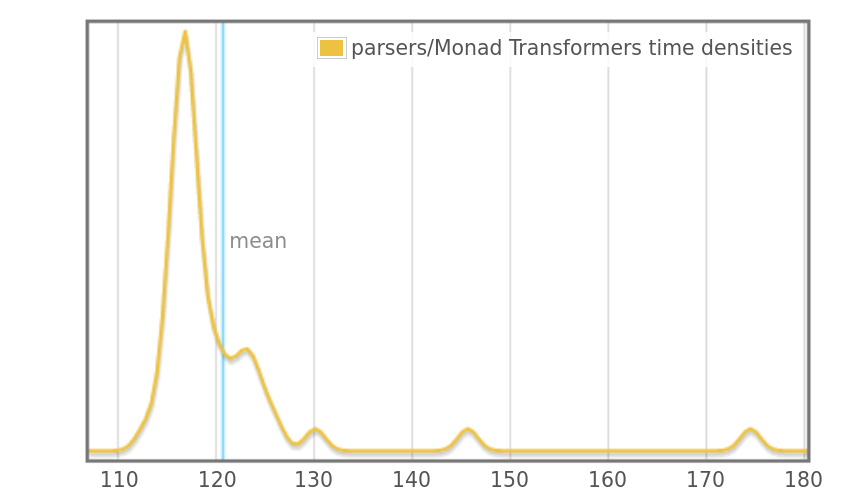
\includegraphics[scale=0.4]{images/monad-trans.png}
      \caption{Monad transformers parsers benchmark}
      \label{mtlParserBench}
      \end{figure}

      The benchmarking was performed for a parser of a Markdown"/like language
      implemented using this library. The benchmarked action was parsing of a
      file of size about 3 kilobytes. The benchmark, together with the source code
      of the library and the parser may be found in the library's GitHub
      repository~\cite{mdParse}.


    \section{Conclusion}

    Overall, a concept of monad transformers has a considerable convenience in programming due to
    its maturity and popularity. However, this
    approach lacks flexibility, doesn't permit stacks with several homogeneous
    effects (for instance, multiple~\texttt{StateT} transformers) without
    losing automatic lifting (~\texttt{lift}) and requires boilerplate
    type class instance declaration.

    The next chapter considers different method of constructing parser combinators: one
    based on algebraic effects and effects handlers --- an alternative framework of construction of effectful computation. We are going to present two prototype
    parser combinators libraries, one embedded into Haskell by means of extensible
    effects, and another implemented in Frank --- an experimental programming language
    with native support foe algebraic effects.